\section*{Introduction}

\subsection*{Introduction}

\begin{frame}{Le contrôle moteur}
    \begin{block}{But}
        Amener un {\em système mécanique} d'un {\em état} initial à un état désiré
        \begin{center}
            \includegraphics[width=.40\linewidth]{fig/path}
        \end{center}
    \end{block}
\end{frame}

\begin{frame}{La boucle de contrôle}
    \begin{center}
        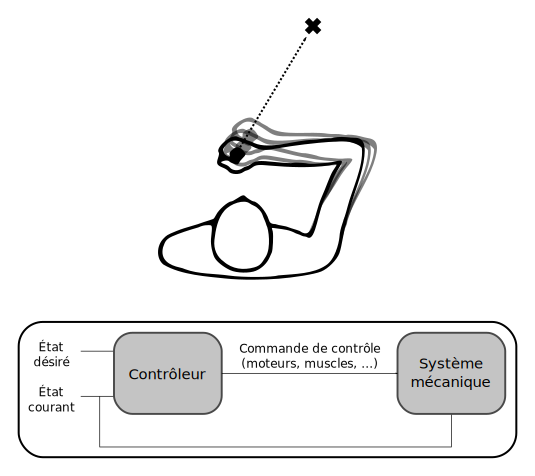
\includegraphics[width=.70\linewidth]{fig/ctrl2}
    \end{center}
\end{frame}

\begin{frame}{Nos objectifs}
    \begin{columns}
        \begin{column}{0.50\textwidth}
            \begin{itemize}
                \item Faire du contrôle moteur sur un système complexe 
                \item Générer des mouvements réalistes et efficaces en reproduisant les propriétés connues du contrôle moteur humain
                %\item Faire un contrôleur pouvant être appris avec les techniques actuelles d'IA
            \end{itemize}
        \end{column}
        \begin{column}{0.50\textwidth}
            \begin{center}
                \includegraphics[width=.95\linewidth]{fig/icub_light}
            \end{center}
        \end{column}
    \end{columns}
\end{frame}

\subsection*{Problématique}

\begin{frame}{Problèmes}
    \begin{small}
        Les techniques actuelles ne permettent pas de remplir ces 2 conditions à la fois~:
        ~\\
        \begin{columns}
            \begin{column}{0.70\textwidth}
                \begin{block}{Robotique}
                    Systèmes complexes mais mouvement pas \og{}réaliste\fg{} et peu \og{}efficace\fg{} %pas \og{}human like\fg{} $[$RMRC, Toussaint, ...$]$
                \end{block}
                \begin{block}{Contrôle moteur}
                    Systèmes simples seulement %$[$Rigoux et Guigon, Todorov, ...$]$
                \end{block}
                %\begin{block}{IA - Apprentissage}
                %    Systèmes simples seulement (\og{}malédiction de la dimensionalité\fg{})
                %    %\og{}Malédiction de la dimensionalité\fg{} en apprentissage
                %\end{block}
            \end{column}
            \begin{column}{0.30\textwidth}
                \begin{center}
                    \includegraphics[width=.95\linewidth]{fig/asimo}
                \end{center}
            \end{column}
        \end{columns}
    \end{small}
\end{frame}

%\subsection{Problématique}
%
%%%%%%%%%%%%%%%%%%%%%%%%%%%%%%%%%%%%%%%%
%
%\begin{frame}{Introduction}
%    \begin{figure}
%        \centering
%        \subfigure[Corps humain]{\includegraphics[width=.50\linewidth]{fig/arm4}}~~~
%        \subfigure[Système mécanique poly-articulé]{\includegraphics[width=.50\linewidth]{fig/arm1}}
%    \end{figure}
%\end{frame}
%
%\begin{frame}{Introduction}
%    \begin{small}
%        \begin{itemize}
%            \item Système mécanique défini par un état (vitesse position)
%            \item L'état peut être décrit dans plusieurs espaces
%        \end{itemize}
%    \end{small}
%    \begin{figure}[ht]
%        \centering
%        \input{tikz/tikz_slides_arm_space.tex}
%    \end{figure}
%    \begin{small}
%    Notations : état  $\jstate = \begin{pmatrix} \dq & \q \end{pmatrix}^T$ et 
%    $\ostate = \begin{pmatrix} \dx & \x \end{pmatrix}^T$
%    \end{small}
%\end{frame}
%
%%\begin{frame}{Problématique}
%%    Redondant dans l'espace de la tâche
%%    \begin{center}
%%        \includegraphics[width=.40\linewidth]{fig/arm2}
%%    \end{center}
%%\end{frame}
%
%\begin{frame}{Problématique}
%    \begin{block}{Une question clé}
%        Pourquoi réalise-t-on tel mouvement plutôt qu'un autre~? $[$Bernstein~67$]$
%    \end{block}
%    \begin{center}
%        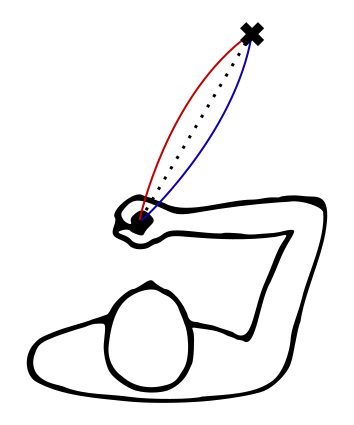
\includegraphics[width=.40\linewidth]{fig/paths}
%    \end{center}
%\end{frame}
%
%%%%%%%%%%%%%%%%%%%%%%%%%%%%%%%%%%%%%%%%
%
%\begin{frame}{Un début de réponse\dots}
%    \begin{block}{Un processus d'optimisation~?}
%        \begin{itemize}
%            \item Pourquoi deux tâches identiques produisent des mouvements différents ?
%            \item Peut-on quantifier ces variations ?
%        \end{itemize}
%    \end{block}
%    Plusieurs propriétés du contrôle moteur ont été identifiées
%    \begin{block}{Principes clés~:}
%        \begin{itemize}
%            \item Minimisation de la variance au point final
%            \item Principe d'intervention minimum
%        \end{itemize}
%    \end{block}
%\end{frame}
%
%%%%%%%%%%%%%%%%%%%%%%%%%%%%%%%%%%%%%%%%
%
%\begin{frame}{Des pistes d'améliorations}
%    Contrôleur de $[$Rigoux et Guigon 11$]$
%    \begin{itemize}
%        \item Reproduit les propriétés du contrôle moteur
%        \item Mais\dots optimise les actions musculaires $\Rightarrow$ trop lent
%    \end{itemize}
%    Regarder le problème sous un autre angle~:
%    \begin{itemize}
%        \item Cinématique
%        \item Dynamique
%        \item Actionnement
%    \end{itemize}
%    Peut-on optimiser sur un plus petit espace ?
%\end{frame}

